\documentclass[a4paper]{article}

\usepackage{times}
\usepackage{tikz}
\usepackage[margin=0cm]{geometry}
\usepackage{graphicx}
\usepackage{anyfontsize}
\usepackage{fancyhdr}
\usepackage{indentfirst}
\usepackage{amsmath}
\usepackage[spanish]{babel}
\usepackage[utf8]{inputenc}
\usepackage{titlesec}
\usepackage{booktabs}
\usepackage{multicol}

\author{}
\date{}
\title{}

\begin{document}
\thispagestyle{empty}

\begin{tikzpicture}[remember picture, overlay]
    \pgftransformshift{\pgfpoint{0cm}{0cm}}
    \draw [line width=2pt](1cm,-1cm) -- (1cm,-27.7cm) -- (14cm, -27.7cm) -- (14cm, -1cm) -- (1cm, -1cm);
    \draw[line width=2pt] (15cm, -27.7cm) -- (19cm,-27.7cm) -- (19cm, -1cm) -- (15cm, -1cm) --  (15cm, -27.7cm);
    \node [line width=2pt] at (17cm, -3.5cm) {
\includegraphics[width=3cm]{/home/marcosgatica/Imágenes/utn.png}};
		\node [line width=2pt] at (7.5cm, -7.5cm) {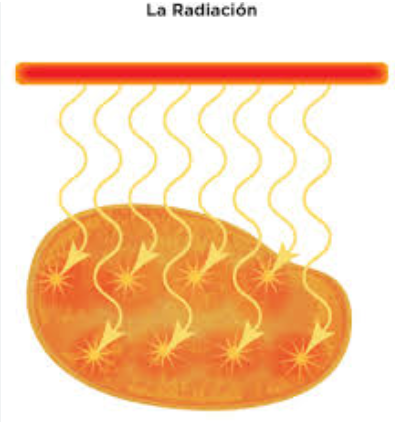
\includegraphics[width=6cm]{./imagenCaratula.png}};
    \node at (17cm, -7cm) {\scalebox{5}{\textbf{U}}};
    \node at (17cm, -9cm) {\scalebox{5}{\textbf{T}}};
    \node at (17cm, -11cm) {\scalebox{5}{\textbf{N}}};
    \node at (17cm, -14cm) {\scalebox{5}{\textbf{F}}};
    \node at (17cm, -16cm) {\scalebox{5}{\textbf{R}}};
    \node at (17cm, -18cm) {\scalebox{5}{\textbf{C}}};
    \node at (7.5cm, -12cm) {\scalebox{2.5}{\textbf{RADIACIÓN TÉRMICA}}};

    \node at (7.5cm, -24cm) {\begin{minipage}[c]{12cm}
        \raggedright
        \vspace{1.5cm}
        \fontsize{14}{14}\selectfont \textbf{Autor:} Marcos Raúl Gatica. \\
        \fontsize{14}{14}\selectfont \textbf{Curso:} 2R1. \\
        \fontsize{14}{14}\selectfont \textbf{Asignatura:} Física Electrónica. \\
        \fontsize{14}{14}\selectfont \textbf{Institución:} Universidad Tecnológica Nacional - Facultad Regional de Córdoba. \\

    \end{minipage}};

\end{tikzpicture}

\renewcommand{\normalsize}{\fontsize{12}{18}\selectfont}
\newgeometry{margin=1cm}
\fancyhf{}
\renewcommand{\headrulewidth}{0pt}
\renewcommand{\footrulewidth}{0pt}
\fancyfoot[R]{\textit{Gatica M. - Leg. 402006 - 2R1 pág. \thepage}}
\setlength{\footskip}{0pt}

\titleformat{\section} {\fontsize{12}{12}\bfseries}{\thesection.}{0.5em}{\underline}

\newpage
\newpage

\thispagestyle{empty}
\setcounter{page}{0}
\tableofcontents

\newpage
\thispagestyle{fancy}

\begin{multicols}{2}
    \flushbottom
    \section{INTRODUCCIÓN}
        \subsection{La radiación térmica}
            \indent Se entiende como la radiación térmica al modo de transmitir calor de un sistema (la superficie de un cuerpo) al entorno. No requiere un medio para transmitirse, aunque es más eficaz la transmisión en el vacío. \\
            \indent Una superficie calentada a un temperatura finita interactua con el medio a menor temperatura y comienza la transmisión de calor, esto último es conocido como la radiación que emite un objeto más caliente que su entorno hasta alcanzar el equilibrio térmico. \\
            \indent La radiación que emite un sólido más caliente que su entorno se conoce como emisividad (\textbf{E}), proviene de la energía interna y la velocidad a la que la energía es emitida por la materia por su unidad de área (\textit{$\frac {W} {m^2}$}). \\

        \subsection{Radiación y las longitudes de onda}
            \indent La radiación térmica que emite un cuerpo caliente representa varias longitudes de onda. Gráficamente se puede ver que cada curva representa la variación de emisión monocromática con la long. de onda $\lambda$ \\

            \begin{tikzpicture}[remember picture, overlay]
                \node at (2.75cm, -2cm) {
                    \begin{minipage}[c]{3cm}
                    \includegraphics[width = 5.5cm]{./radiaciónTermVSLambda.png}
            \end{minipage}};
            \end{tikzpicture}
        \vspace{4.8cm}

        \subsection{Experimento y objetivos}
            \indent El objetivo de este desarrollo de laboratorio es determinar la radiación térmica que emanan los siguientes materiales: \\
            \begin{itemize}
                \setlength{\itemsep}{0pt}
                \item Plomo 
                \item Aluminio anodizado
                \item Aluminio
                \item Cobre 
                \item Chapa negra
            \end{itemize}
        
            \indent Complementario a esto, se tomará uno de los elementos seleccionados de la lista anterior para medir la radiación a cierta distancia del mismo con el fin de evaluar cómo el entorno del laboratorio influye en las mediciones de radiación. \\

     \section{REQUERIMIENTOS}
        El desarrollo del trabajo en el laboratorio requirió de los siguientes elementos:
        \subsection{El cubo de Leslie}
            \indent El cubo de Leslie permite medir y/o mostrar la energía radiada por diversos materiales en contacto con el dispositivo. \\
            \indent La electrónica asociada del dispositivo empleado (con trasmisores LM-335, transductores pasivos y activos) permite obtener una sensibilidad de \textit{10mV x 1\textdegree K} \\
            %IMAGEN DEL APARATO
            \indent \textit{Nota: debido a un desperfecto en el instrumento, se optó por medir la temperatura de los materiales de otra forma. Naturalmente el dispositivo tiene una salida para leer los mV de la relación anteriormente mencionada.}
        \subsection{Sensor de radiación Pasco}
            \indent Este sensor lee la radiación térmica emitida por un cuerpo y devuelve un valor en mV en relación a la cantidad de mW detectados (\textit{22mV x mW}). \\
            \begin{tikzpicture}[remember picture, overlay]
                \node at (4.75cm, -3.25cm) {
                    \begin{minipage}[c]{3cm}
                        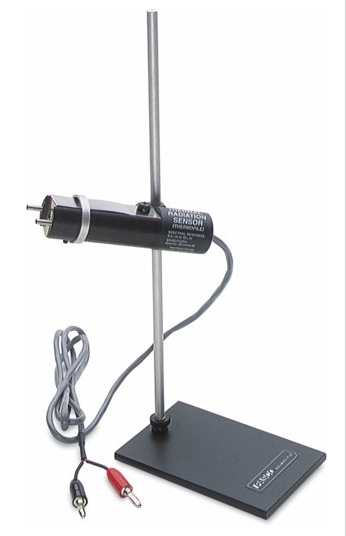
\includegraphics[width = 3.5cm]{./sensorPasco.png}
                    \end{minipage}};
            \end{tikzpicture}
            \vspace{6.5cm}

        \subsection{Multímetros}
            \indent El experimento requirió de dos multímetros: uno como solución al problema del cubo de Leslie, con el cual se realizaron las mediciones de temperatura a la placa en grados Celsius usando sondas; y el restante para medir los mV del sensor Pasco.
            \begin{tikzpicture}[remember picture, overlay]
                \node at (-4.5cm, -3cm) {
                    \begin{minipage}[c]{3cm}
                        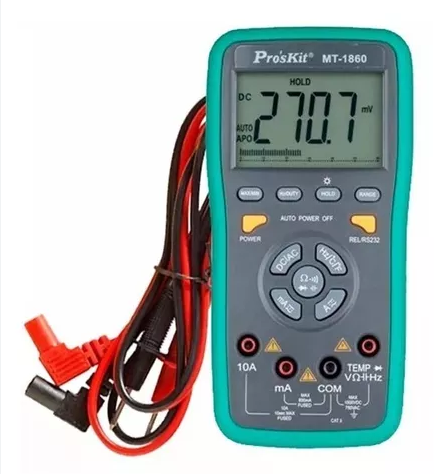
\includegraphics[width = 4cm]{./multimetro.png}
                    \end{minipage}};
            \end{tikzpicture}
            \vspace{5cm}
    \section{PROCEDIMIENTO}
        \subsection{Medición de radiación de materiales}

        \indent Se colocó cada placa del material en cuestión sobre la superficie del cubo de Leslie con el fin de que esta se calentase. Las siguientes tablas muestran las series de mediciones realizadas, de cada muestra, donde se registraron datos de evolución del sensor Pasco hasta una temperatura de equilibrio (donde la placa no subía más de temperatura en contacto con el cubo de Leslie):

        \newpage
        \thispagestyle{fancy}

        \begin{center}
            \textit{Aluminio} 

            \vspace{2.5mm}

            \begin{tabular}{ c  c  c }
                \toprule
                 N \textdegree & Sensor Pasco (mV) & Temperatura (\textdegree C) \\ 
                 \midrule
                      1   &   1,4     &   51,7 \\ 
                      2   &   1,4     &   50,8 \\ 
                      3   &   1,3     &   49,6 \\ 
                      4   &   1,3     &   48,6 \\ 
                      5   &   1,2     &   47,6 \\ 
                      6   &   1,1     &   46,6 \\ 
                      7   &   1,0     &   45,6 \\ 
                      8   &   1,0     &   44,6 \\ 
                      9   &   0,9     &   43,6 \\ 
                      10  &   0,8     &   42,6 \\ 
                      11  &   0,8     &   41,6 \\ 
                      12  &   0,7     &   40,6 \\ 
                      13  &   0,6     &   39,6 \\ 
                      14  &   0,6     &   38,6 \\ 
                      15  &   0,5     &   37,6 \\ 
                      16  &   0,4     &   36,4 \\ 
                \bottomrule
            \end{tabular}
       
            \vspace{5mm}

            \textit{Cobre} 

            \vspace{2.5mm}

            \begin{tabular}{ c  c  c }
                \toprule
                 N \textdegree & Sensor Pasco (mV) & Temperatura (\textdegree C) \\ 
                 \midrule
                     1   &   1,7     &   51,3 \\ 
                     2   &   1,6     &   51,5 \\ 
                     3   &   1,5     &   50,6 \\ 
                     4   &   1,4     &   49,6 \\ 
                     5   &   1,3     &   48,6 \\ 
                     6   &   1,2     &   47,1 \\ 
                     7   &   1,1     &   45,9 \\ 
                     8   &   1,0     &   44,7 \\ 
                     9   &   0,9     &   43,2 \\ 
                     10  &   0,8     &   40,7 \\ 
                     11  &   0,7     &   40,3 \\ 
                     12  &   0,6     &   38,8 \\ 
                \bottomrule
            \end{tabular}
            
            \vspace{5mm}

            \textit{Aluminio anodizado} 

            \vspace{2.5mm}

            \begin{tabular}{ c  c  c }
                \toprule
                N \textdegree & Sensor Pasco (mV) & Temperatura (\textdegree C) \\
                \midrule
                    1   & 2,9  & 50  \\ 
                    2   & 2,7  & 49  \\ 
                    3   & 2,6  & 48  \\ 
                    4   & 2,4  & 47  \\ 
                    5   & 2,2  & 46  \\ 
                    6   & 2    & 45  \\ 
                    7   & 1,9  & 44  \\ 
                    8   & 1,8  & 43  \\ 
                    9   & 1,6  & 42  \\ 
                    10   & 1,5  & 41 \\ 
                    11  & 1,3  & 40  \\ 
                \bottomrule
            \end{tabular}

            \columnbreak

            \textit{Plomo} 

            \vspace{2.5mm}

            \begin{tabular}{ c  c  c }
                \toprule
                N \textdegree & Sensor Pasco (mV) & Temperatura (\textdegree C) \\
                \midrule
                1   &  3,5 &  51  \\
                2   &  3,3 &  50,5 \\
                3   &  3,2 &  50 \\
                4   &  3   &  49 \\
                5   &  2,9 &  48 \\ 
                6   &  2,7 &  47 \\ 
                7   &  2,5 &  46 \\ 
                8   &  2,4 &  45 \\ 
                9   &  2,2 &  44 \\
                10  &  2   &  43 \\ 
                11  &  1,9 &  42 \\ 
                12  &  1,8 &  41 \\ 
                13  &  1,6 &  40 \\
                14  &  1,4 &  39 \\ 
                15  &  1,3 &  38 \\
                16  &  1,1 &  37 \\
                \bottomrule
            \end{tabular}
            
            \vspace{5mm}

            \textit{Chapa negra} 

            \vspace{2.5mm}

            \begin{tabular}{ c  c  c }
                \toprule
                N \textdegree & Sensor Pasco (mV) & Temperatura (\textdegree C) \\
                \midrule
                    1   &   3,8 &   51 \\
                    2   &   3,6 &   50,4 \\
                    3   &   3,5 &   49,5 \\
                    4   &   3,3 &   48,8 \\
                    5   &   3,1 &   47,5 \\
                    6   &   3   &   46,6 \\
                    7   &   2,9 &   45,8 \\
                    8   &   2,7 &   45,1 \\
                    9   &   2,2 &   42,4 \\
                    10  &   2   &   41,5 \\
                    11  &   1,9 &   40,4 \\
                    12  &   1,7 &   39,4 \\
                    13  &   1,5 &   38,5 \\
                    14  &   1,4 &   37,9 \\
                \bottomrule
            \end{tabular}

        \end{center}

        \subsection{Gráfico de tendencia}
            \indent En este apartado, usando los datos obtenidos de las mediciones, se realizará un gráfico de la radiación térmica en función de la temperatura de cada material.
    \end{multicols}
\end{document}


